% This is "sig-alternate.tex" V2.1 April 2013
% This file should be compiled with V2.5 of "sig-alternate.cls" May 2012
%
% This example file demonstrates the use of the 'sig-alternate.cls'
% V2.5 LaTeX2e document class file. It is for those submitting
% articles to ACM Conference Proceedings WHO DO NOT WISH TO
% STRICTLY ADHERE TO THE SIGS (PUBS-BOARD-ENDORSED) STYLE.
% The 'sig-alternate.cls' file will produce a similar-looking,
% albeit, 'tighter' paper resulting in, invariably, fewer pages.
%
% ----------------------------------------------------------------------------------------------------------------
% This .tex file (and associated .cls V2.5) produces:
%       1) The Permission Statement
%       2) The Conference (location) Info information
%       3) The Copyright Line with ACM data
%       4) NO page numbers
%
% as against the acm_proc_article-sp.cls file which
% DOES NOT produce 1) thru' 3) above.
%
% Using 'sig-alternate.cls' you have control, however, from within
% the source .tex file, over both the CopyrightYear
% (defaulted to 200X) and the ACM Copyright Data
% (defaulted to X-XXXXX-XX-X/XX/XX).
% e.g.
% \CopyrightYear{2007} will cause 2007 to appear in the copyright line.
% \crdata{0-12345-67-8/90/12} will cause 0-12345-67-8/90/12 to appear in the copyright line.
%
% ---------------------------------------------------------------------------------------------------------------
% This .tex source is an example which *does* use
% the .bib file (from which the .bbl file % is produced).
% REMEMBER HOWEVER: After having produced the .bbl file,
% and prior to final submission, you *NEED* to 'insert'
% your .bbl file into your source .tex file so as to provide
% ONE 'self-contained' source file.
%
% ================= IF YOU HAVE QUESTIONS =======================
% Questions regarding the SIGS styles, SIGS policies and
% procedures, Conferences etc. should be sent to
% Adrienne Griscti (griscti@acm.org)
%
% Technical questions _only_ to
% Gerald Murray (murray@hq.acm.org)
% ===============================================================
%
% For tracking purposes - this is V2.0 - May 2012

\documentclass{sig-alternate-05-2015}

%%%%%%%%%%%%%%%%%%%%%%%%%
%                              My Commands
\newcommand{\bi}{\begin{itemize}}
\newcommand{\ei}{\end{itemize}}
\newcommand{\be}{\begin{enumerate}}
\newcommand{\ee}{\end{enumerate}}
\newcommand{\ii}{\item}
\newtheorem{Def}{Definition}
\newtheorem{Lem}{Lemma}
\usepackage{algorithm}
\usepackage{algorithmicx}
\usepackage{algpseudocode}

\usepackage{graphicx}
\graphicspath{%
        {converted_graphics/}
        {./images/}
}
\usepackage{times}

% 				End of My Commands
%%%%%%%%%%%%%%%%%%%%%%%%%

\begin{document}

% Copyright
\setcopyright{acmcopyright}
%\setcopyright{acmlicensed}
%\setcopyright{rightsretained}
%\setcopyright{usgov}
%\setcopyright{usgovmixed}
%\setcopyright{cagov}
%\setcopyright{cagovmixed}


% DOI
\doi{10.475/123_4}

% ISBN
%\isbn{123-4567-24-567/08/06}

%Conference
%\conferenceinfo{PLDI '13}{June 16--19, 2013, Seattle, WA, USA}

\acmPrice{\$15.00}

%
% --- Author Metadata here ---
\conferenceinfo{BIGDAS 2015}{Jeju Island, Republic of Korea}
%\CopyrightYear{2007} % Allows default copyright year (20XX) to be over-ridden - IF NEED BE.
%\crdata{0-12345-67-8/90/01}  % Allows default copyright data (0-89791-88-6/97/05) to be over-ridden - IF NEED BE.
% --- End of Author Metadata ---

\title{Flying KIWI: Design of Approximate Query Processing Engine for Interactive Data Analytics at Scale }

\numberofauthors{1} 

\author{
% 1st. author
\alignauthor
Sung-Soo Kim, Moonyoung Chung, Taewhi Lee and Jongho Won \\
       \affaddr{Electronics and Telecommunications Research Institute (ETRI)}\\
       \affaddr{218 Gajeong-ro, Yuseong-gu, Daejeon}\\
       \affaddr{South Korea}\\
       \email{\{sungsoo, mchung, taewhi, jhwon\}@etri.re.kr}
}

% There's nothing stopping you putting the seventh, eighth, etc.
% author on the opening page (as the 'third row') but we ask,
% for aesthetic reasons that you place these 'additional authors'
% in the \additional authors block, viz.
\additionalauthors{Additional authors: John Smith (The Th{\o}rv{\"a}ld Group,
email: {\texttt{jsmith@affiliation.org}}) and Julius P.~Kumquat
(The Kumquat Consortium, email: {\texttt{jpkumquat@consortium.net}}).}
\date{30 July 1999}
% Just remember to make sure that the TOTAL number of authors
% is the number that will appear on the first page PLUS the
% number that will appear in the \additionalauthors section.

\maketitle
\begin{abstract}
We present a architecture of approximate query processing engine for interactive big data analytics. 
In this paper, we summarize the design, development, and current state of deployment of the next generation of SQL-on-Hadoop system: KIWI.
\end{abstract}


%\ccsdesc[500]{Information systems~Data management systems}
%\ccsdesc[300]{Data management systems~Query optimization}
\ccsdesc[200]{Data management systems engines~Parallel and distributed DBMSs}
\ccsdesc[100]{Parallel and distributed DBMSs~Relational parallel and distributed DBMSs}


%
% End generated code
%

%
%  Use this command to print the description
%
\printccsdesc

% We no longer use \terms command
%\terms{Theory}

\keywords{Approximate Query Processing; Big Data Analytics; Random Sampling}

\section{Introduction}
A \textit{data warehouse} (DW) is the collection of processes and data whose overarching purpose is to support the business with it analysis and decision-making. 
SQL-on-Hadoop is a class of "Big Data" analytics systems that combine established SQL-style querying with Hadoop-based data warehouse.

One of the earliest efforts to combine SQL and Hadoop resulted in the Hive data warehouse, which featured HiveQL software for translating SQL-like queries into MapReduce jobs. Other tools that help support SQL-on-Hadoop include Impala, Presto, SparkSQL, Tajo, Impala, Drill, Hadapt, HAWQ, BigSQL, Stinger, and Hive on Tez \cite{Floratou:2014}.
% \cite{Babcock:2003, Chaudhuri:2007, Zeng:2015, Floratou:2014, Agarwal:2014, Agarwal:2013}.
%When considering SQL-on-Hadoop, the most fundamental question is: What is the right tool for the job? 
For \textit{interactive queries} that require a few seconds (or even milliseconds) of response time, MapReduce (MR) is the wrong choice, since MR is often suitable for \textit{batch processing}. 
%On the other hand, for queries that require massive scale and runtime fault tolerance, an MR framework works well. 
%MR was built for large-scale processing on big data, viewed mostly as \textit{batch processing}.
%To provide an effective environment for big data analysis, we believe that processing systems will need to support both SQL and complex analytics efficiently, and to provide fine-grained fault recovery across both types of operations.
In order to provide an effective environment for big data analysis, we believe that SQL-on-Hadoop systems will need to support both \textit{interactive} analytics and \textit{deep} analytics based on massively \textit{batch} processing. 
\textit{KIWI} is a  SQL-on-Hadoop system, which runs on hundreds of machines in existing Hadoop cluster.
It is decoupled from the underlying storage engine, unlike traditional database management systems where the query processing and the underlying storage engine are components of a single tightly-coupled system.
The ultimate goal of our work is to provide a SQL-on-Hadoop system, which can support interactive analytics as well as deep (batch) analytics. \textit{Flying KIWI} is an \textit{approximate} query processing (AQP) engine in order to support interactive analytics. Flying KIWI provides an approximate answer with an error bar, which is calculated by error estimation. Error estimation in AQP can be categorized into two main approaches, such as closed-form and bootstrap.
%\textit{Bootstrap} is a powerful method for approximating unknown distributions. 
Closed-form error estimation is often used for common aggregate functions in a SQL query, such as \texttt{COUNT, SUM, AVG}, etc. 
Bootstrap consists in a simple Monte Carlo procedure, however, this requires the computational overhead. 
\textit{Analytical bootstrap} has been proven equivalent to the simulation-based bootstrap, but avoids the computational overhead \cite{Agarwal:2014}.  

\noindent
\textbf{Main contributions:} 
%We present a novel system architecture for approximate query processing engine for interactive big data analytics. 
The contributions of our work can be summarized as follows. 
\bi
\ii \textit{Dual-Mode Analytics}: 
The proposed SQL-on-Hadoop system supports \textit{interactive} analytics as well as MR-based \textit{batch} processing in the unified KIWI architecture.
\ii \textit{Approximate Query Processing}: 
We introduce a progressive error estimation method to support online aggregation using the \textit{Flying KIWI}.
\ei
\section{System Architecture}
This section focuses on the overall architecture for approximate query processing engine and describes each module in the system architecture. Figure \ref{fig:architecture} shows the high-level architecture of our system, which can be divided into two main blocks, such as \textit{query compilation} block and \textit{query execution} block.
\begin{figure}[htb]
        \centering
        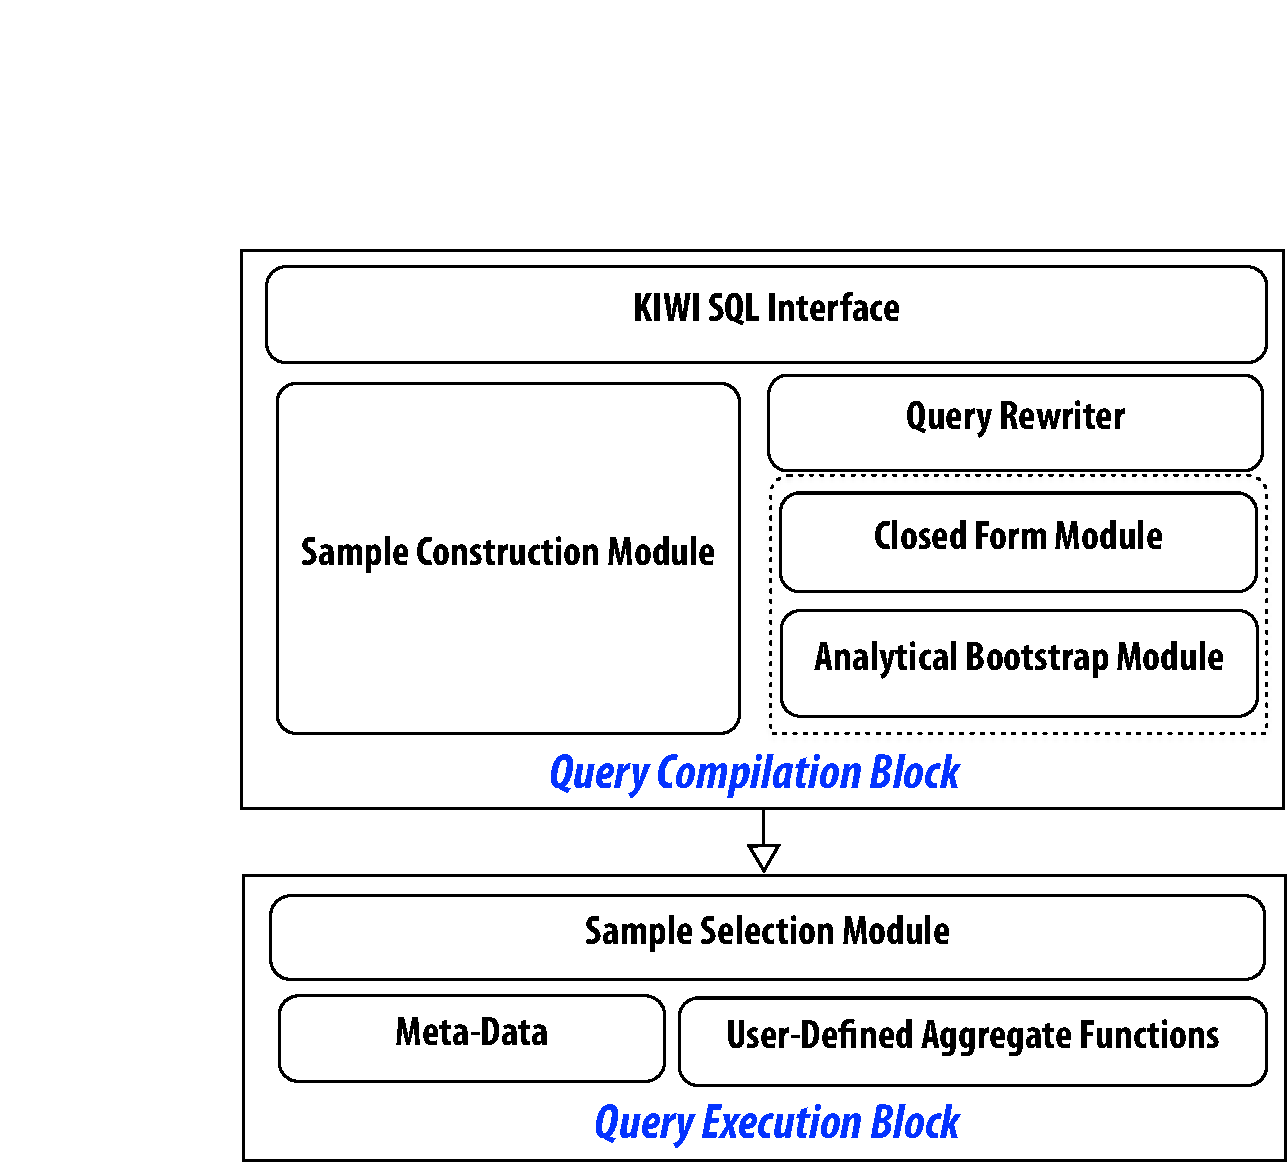
\includegraphics[width=0.3\textwidth]{sys-architecture.pdf}
        \caption{System Architecture.}
        \label{fig:architecture}
\end{figure}

\noindent
\textbf{Query Compilation Block:} 
This block performs transparently compiling, checking and rewriting the query to support error estimation using closed forms or analytical bootstrap. The compiler generates a query plan expressed in relational algebra from the a given SQL query. 
%Error estimation in AQP can be categorized into two main approaches, such as closed-form and bootstrap.
%\textit{Bootstrap} is a powerful method for approximating unknown distributions. 
%Closed-form error estimation is often used for common aggregate functions in a SQL query, such as \texttt{COUNT, SUM, AVG}, etc. 
%Bootstrap consists in a simple Monte Carlo procedure, however, this requires the computational overhead. 
%\textit{Analytical bootstrap} has been proven equivalent to the simulation-based bootstrap, but avoids the computational overhead. % \cite{Agarwal:2014}.  
The query rewriter takes into consideration the user-specified quality measures, and rewrites the plan into a new logical query plan.

\noindent
\textbf{Query Execution Block:} 
The execution block evaluates the query augmented with error estimation operations, and providing the accuracy measures in user-specified metrics. 

\subsection{Sample Construction}
Sampling refers to the commonly used technique of evaluating the queries from a small random sample of the original database. The quality of the obtained approximate query answers plays an important role to their utility.

Given a table $T$ with $c$ columns $C_1, ..., C_c$ and $r$ rows, let $S=\{C_i, C_{i+1}, ..., C_{i+k}\}, i \leq i, i+k \leq c$, denote a column set that consists of $k$ columns in $T$. A query $q$ often need to scan fully or partially all data items in a column set $S_q$ of $T$. If data items in $S_q$ have been materialized (stored in a separate area from $T$ independently), for $q$, need to scan only materialized items instead of full table $T$. Because the number of columns in $S_q$ is often much smaller than $c$, scanning would be done much faster.

\begin{figure}[htb]
        \centering
        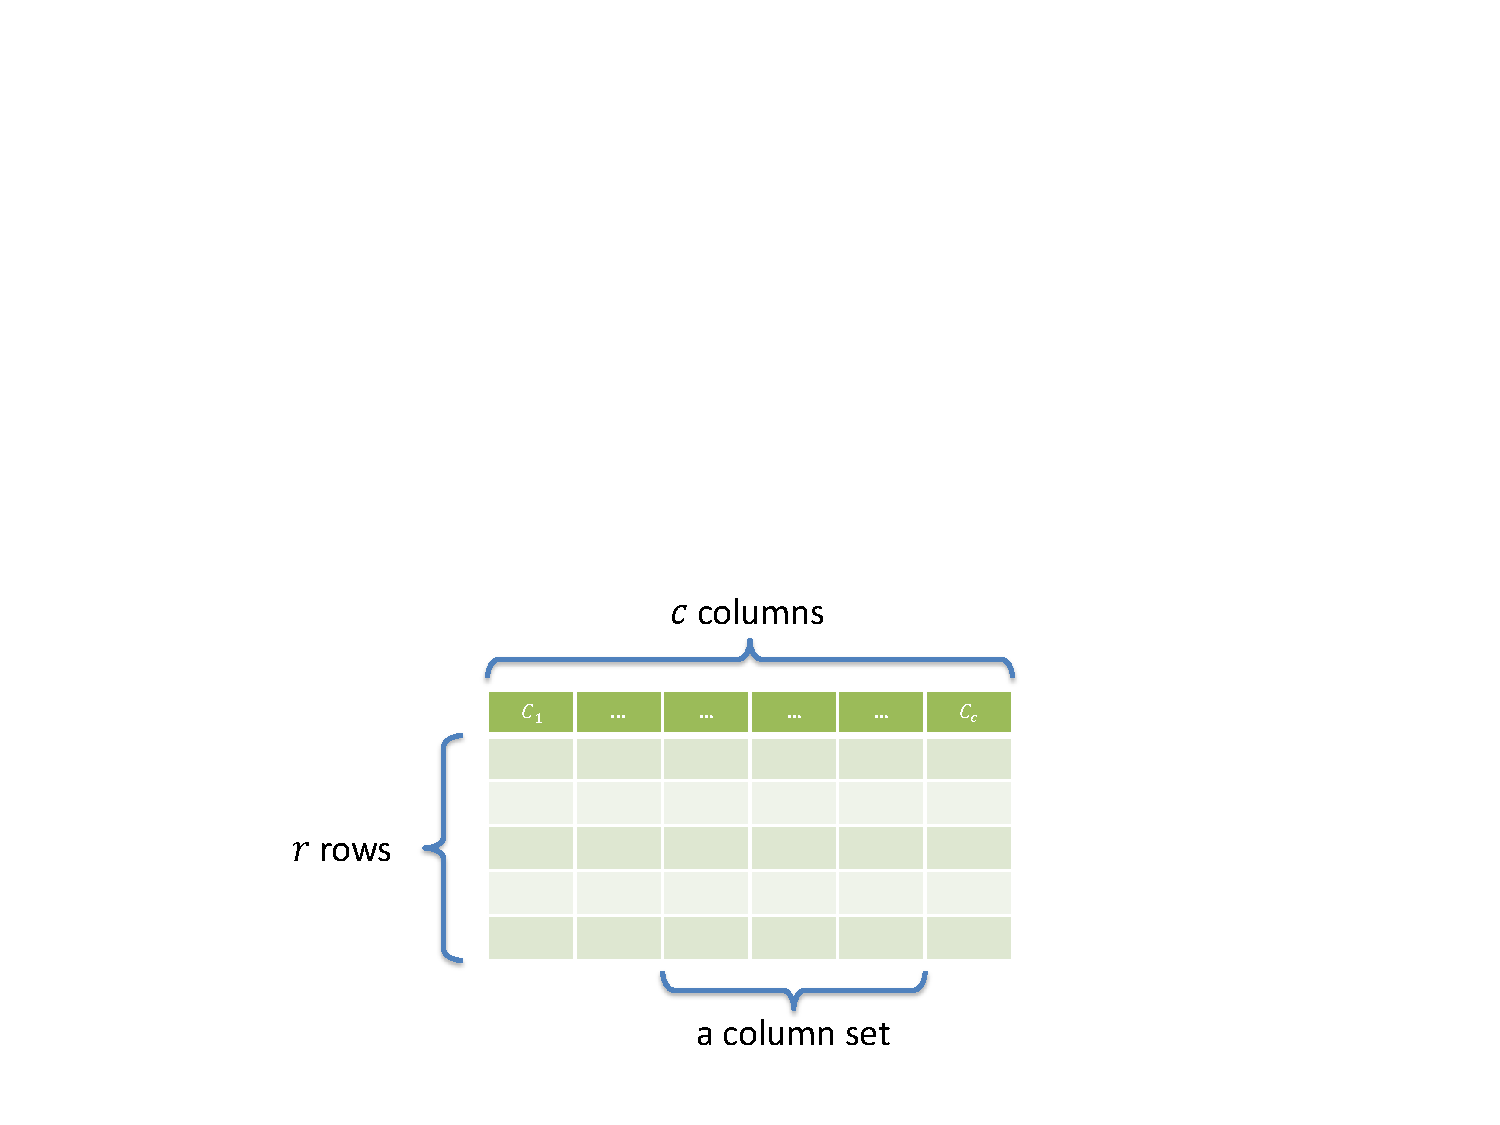
\includegraphics[width=0.3\textwidth]{columnset.pdf}
        \caption{Query Column Set.}
        \label{fig:qcs}
\end{figure}

Let $\xi(T, S)$ be the memory space needed to store all data items in a column set $S$ of a table $T$.
Let $\varphi$ be the storage system's space limit for materialized column sets.
Let $\omega$ be possible column sets of table $T$. 
The sum of the memory space of possible column sets, $\sum_{\forall S_i \in \omega} \xi(T, S)$ is exponentially large.
Let $Q$ is the set of queries issued in the past.
Let $\mathcal{V}(T, S_i)$ be the value obtained for future queries if $S_i$ is materialized.

\noindent
\textbf{Formal problem definition:}  Given a table $T$ and a query $Q$, find a collection of optimal column sets, $S_{opt} = \{S_1, ..., S_k\}$ consisting of $k$ column sets, such that $\sum_{\forall S_i \in \omega} \xi(T, S_i) \leq \omega $ and $\mathcal{V}_{opt} = \sum_{\forall S_i \in \omega} \mathcal{V}(T, S_i) $ is maximized.

\noindent
\textbf{Solution:}
From the set of historical queries $Q_h$ extracts a set of distinct column sets $S_{a}$ that appear in $Q_h$.
$\forall S_i \in S_{a}$, compute $\xi(T, S_i)$, remove from $S_{a}$ if $\xi(T, S_i) > \omega$.
$\forall S_i \in S_{a}$, compute the appearance frequencies $f(S_i)$, remove from $S_{a}$ if $\xi(T, S_i) > \omega$.
Let $n$ be the number of column sets in $S_a$.

For an arbitrary column set $S$, $\xi(T, S)$ can be approximated as
\begin{equation}
\xi(T, S) = r \times \sum_{i=1}^{|S|} \mathcal{I}(C_i)
\end{equation}
where $r$ denotes the number of rows in $T$, 
$|S|$ denotes the number of columns in $S$ 
and $\mathcal{I}(C_i)$ denotes the average size of a data item in $C_i$ 
(e.g., if data type of $C_i$ is double, then $\mathcal{I}(C_i)$ is 8 bytes) .

%\begin{figure}[htb]
%        \centering
%        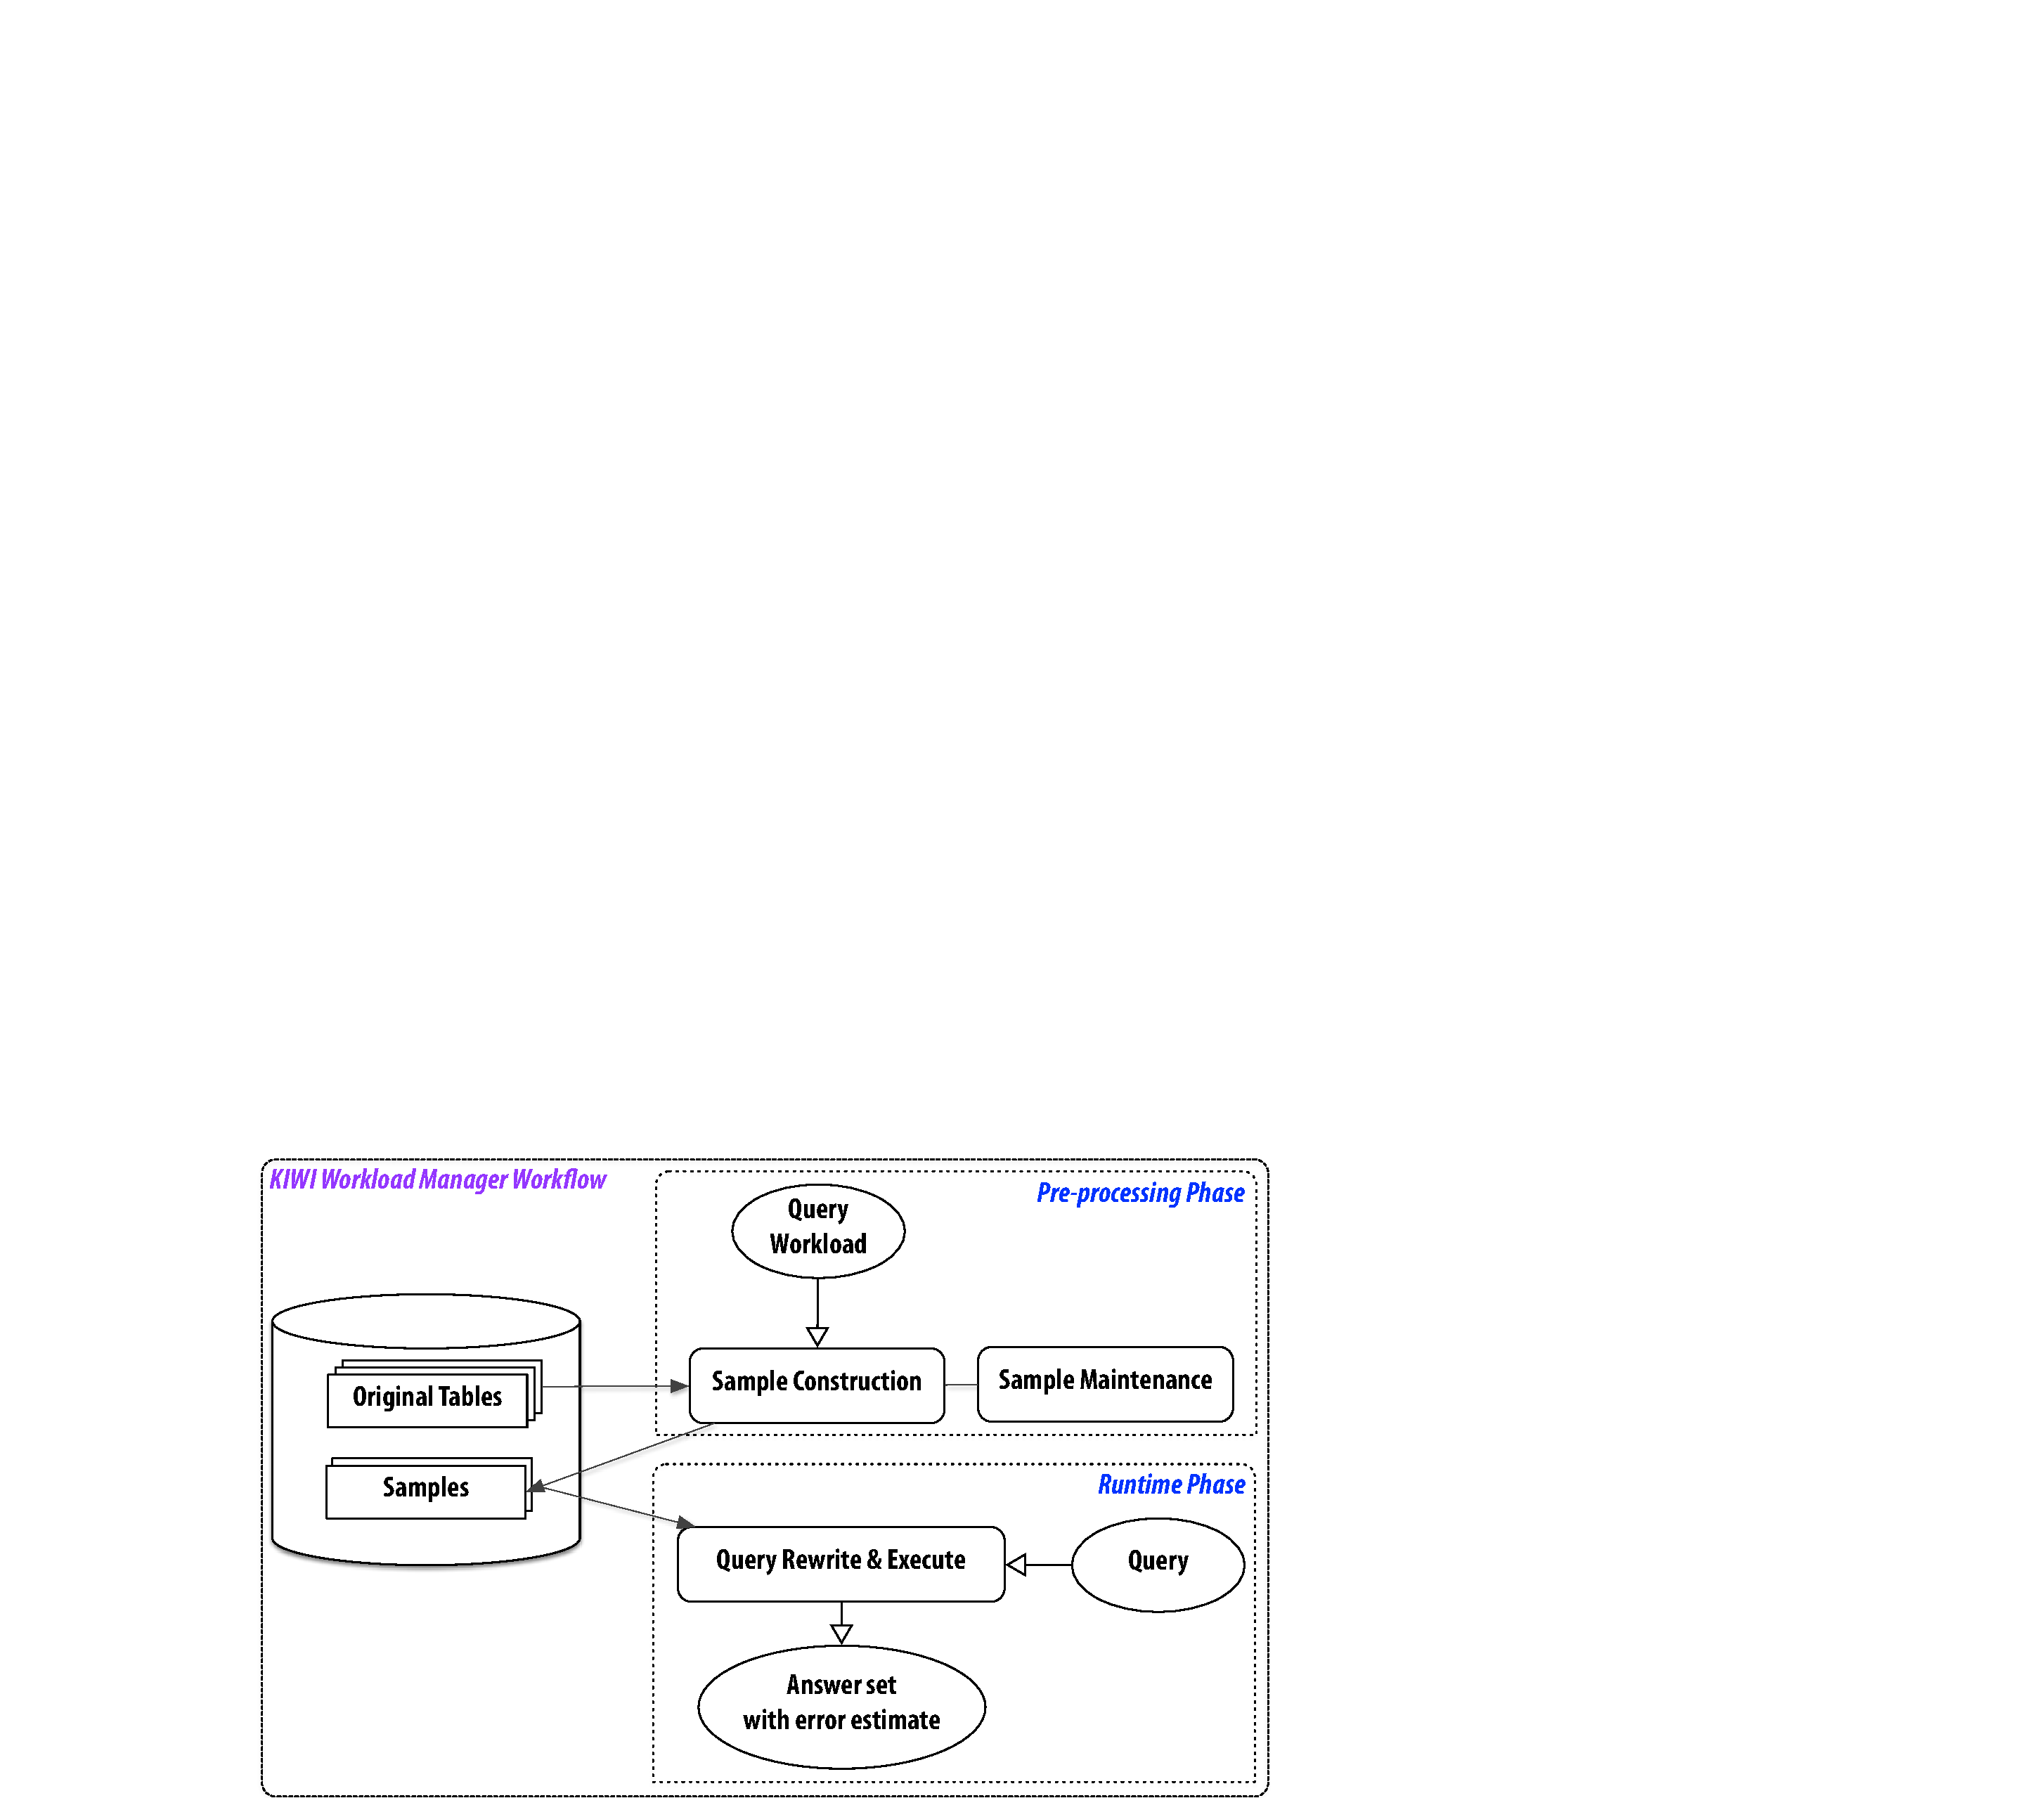
\includegraphics[width=0.48\textwidth]{workflow.pdf}
%        \caption{Approximate Query Processing Workflow.}
%        \label{fig:workflow}
%\end{figure}



\subsection{Column Set Selection}
Online aggregation (OLA) is an attractive technique to respond aggregation queries by computing approximate answers with the error bars over time.

\begin{algorithm}
\caption{Find a optimal column sets.}
\label{algo:columnset}
\begin{algorithmic}[1]
	\Procedure{FindOptimalColumnSets}{$S_a$, $Q$}
	\State List<$S$> $L_{s}$ = \textit{constructColumnSets}($S_a$, $Q$);
	\State $L_{s}$.\textit{sortByAppreanceFrequency}(DESENDING);
	\For{each node $S_j \in L_{s}$ } 
	\If {$\sum_{\forall S_i \in S_{opt}} \xi(T, S_i)  + \xi(T, S_j) > \omega $}
	\Return
	\Else 	
	\State $S_{opt}$.\textit{add}($S_j$); 
	\State $S_a$.\textit{remove}($S_j$); 
	\EndIf
	\EndFor
	\EndProcedure
\end{algorithmic}
\end{algorithm}

%\section{Experiments}
%\section{Related Work}

\section{Conclusion}
We present an architecture of our  system, which support approximate query processing with hadoop-based datawarehouse.
Our work concludes with the following take-away messages:
(1) It is beneficial to have an integrated approximate query processing engine in the KIWI SQL-on-hadoop stack,
(2) \textit{Flying KIWI} is a general purpose system that implements error estimation features of approximate answers and progressive online aggregation frameworks, and
(3) the API is concise and intuitive to use.


















































\small{
\bibliographystyle{abbrv}
\bibliography{sqlonhadoop}
}

\end{document}
